\documentclass[11pt,a4paper,ngerman]{article}
\usepackage[bottom=2.5cm,top=2.5cm]{geometry} 
\usepackage{babel}
\usepackage[utf8]{inputenc} 
\usepackage[T1]{fontenc} 
\usepackage{ae} 
\usepackage{amssymb} 
\usepackage{amsmath} 
\usepackage{graphicx}
\usepackage{fancyhdr}
\usepackage{fancyref}
\usepackage{listings}
\usepackage{xcolor}
\usepackage{paralist}

%\usepackage[pdftex, bookmarks=false, pdfstartview={FitH}, linkbordercolor=white]{hyperref}
\usepackage{fancyhdr}
\pagestyle{fancy}
\fancyhead[C]{CoMa II}
\fancyhead[L]{Übung Nr. 2}
\fancyhead[R]{SoSe 2012}
\fancyfoot{}
\fancyfoot[L]{}
\fancyfoot[C]{\thepage / \pageref{LastPage}}
\renewcommand{\footrulewidth}{0.5pt}
\renewcommand{\headrulewidth}{0.5pt}
\setlength{\parindent}{0pt} 
\setlength{\headheight}{0pt}

\author{Tutor: Sebastian Scherer}
\date{}
\title{Max Wisniewski , Alexander Steen}

\begin{document}

\lstset{language=Pascal, basicstyle=\ttfamily\fontsize{10pt}{10pt}\selectfont\upshape, commentstyle=\rmfamily\itshape\small, keywordstyle=\rmfamily\bfseries, breaklines=true, frame=single, xleftmargin=3mm, xrightmargin=3mm, tabsize=2}

\maketitle
\thispagestyle{fancy}


%% ------------------------------------------------------
%%                     AUFGABE 1
%% ------------------------------------------------------

\section*{Aufgabe 1}
Die Funktion $f: \mathbb{R} \to \mathbb{R}$, mit $x \mapsto \frac{1}{x^2+1}$ soll nach der Methode von Lagrange interpoliert werden. \\

(i) Als quadratisches Polynom: \\ \\
Suche Knotenbasis $\mathfrak{P}$ des $P_2$ mit $\mathfrak{P} = \{\mathfrak{p}_0, \mathfrak{p}_1,\mathfrak{p}_2 \}$.\\
Es gilt:
\begin{eqnarray*}
\mathfrak{p}_k(x) & = & \prod_{i = 0, i \neq k}^{2}{\frac{x-x_i}{x_k-x_i}}\\
\end{eqnarray*}

Stützstellen sind $x_0 = -1$, $x_1 = 0$, $x_2 = 1$, also gilt für die Basis $\mathfrak{P}$:
\begin{eqnarray*}
\mathfrak{p}_0(x) = L_0(x) & = & \prod_{i = 1}^{2}{\frac{x-x_i}{x_k-x_i}} = \frac{x-x_1}{x_0-x_1} \cdot \frac{x-x_2}{x_0-x_2} \\
 & = & \frac{x-0}{(-1) - 0} \cdot \frac{x-1}{(-1) - 1} = -x \cdot \frac{x-1}{-2}
   = \frac{1}{2}(x^2 - x)\\
\mathfrak{p}_1(x) = L_1(x) & = & \prod_{i = 0,i \neq 1}^{2}{\frac{x-x_i}{x_k-x_i}} = \frac{x-x_0}{x_1-x_0} \cdot \frac{x-x_2}{x_1-x_2}\\
 & = & \frac{x-(-1)}{0 - (-1)} \cdot \frac{x-1}{0 - 1} = (x+1) \cdot -(x-1) = -x^2 + 1\\
\mathfrak{p}_2(x) = L_2(x)  & = & \prod_{i = 0}^{1}{\frac{x-x_i}{x_k-x_i}} = \frac{x-x_0}{x_2-x_0} \cdot \frac{x-x_1}{x_2-x_1} \\
 & = & \frac{x-(-1)}{1 - (-1)} \cdot \frac{x-0}{1 - 0} = \frac{x+1}{2} \cdot x
   = \frac{1}{2}(x^2 + x)\\
\end{eqnarray*}

Suche nun das Polynom $p \in P_2$:\\
Das Polynom $p$ wird durch $p = \sum_{k=0}^{2}{f(x_k) \mathfrak{p}_k(x)}$ bestimmt, also gilt:
\begin{eqnarray*}
p & = &\sum_{k=0}^{2}{f(x_k) \mathfrak{p}_k(x)} \\
  & = & f(-1) \cdot \frac{1}{2}(x^2 - x)
  + f(0) \cdot (-x^2 + 1)
  + f(1) \cdot \frac{1}{2}(x^2 + x) \\
  & = & \frac{1}{4}(x^2 - x) + (-x^2 + 1) + \frac{1}{4}(x^2 + x) \\
  & = & -\frac{1}{2}x^2 + 1
\end{eqnarray*}

(ii) Als kubisches Polynom mit zusätzlicher Stelle $x_3 = \frac{1}{2}$. \\ \\
Suche Knotenbasis $\mathfrak{Q}$ des $P_3$ mit $\mathfrak{Q} = \{\mathfrak{q}_0, \mathfrak{q}_1,\mathfrak{q}_2, \mathfrak{q}_3 \}$.\\

$\mathfrak{P}$ wie oben, zusätzliche Stützstelle $x_3 = 1/2$, also gilt für die Basis $\mathfrak{Q}$:
\begin{eqnarray*}
\mathfrak{q}_0(x) & = & \mathfrak{p}_0 \cdot \frac{x-x_3}{x_0-x_3} \\
 & = & \frac{1}{2}(x^2 - x) \cdot \frac{x-1/2}{-3/2}
   = \frac{1}{6}(-2x^3 + 3x^2 - x) \\
\mathfrak{q}_1(x) & = & \mathfrak{p}_1 \cdot \frac{x-x_3}{x_1-x_3} \\
 & = & (-x^2 + 1) \cdot \frac{x-1/2}{-1/2}
   = 2x^3 - x^2 - 2x + 1 \\
\mathfrak{q}_2(x) & = & \mathfrak{p}_2 \cdot \frac{x-x_3}{x_2-x_3} \\
 & = & \frac{1}{2}(x^2 + x) \cdot \frac{x-1/2}{1/2}
   = x^3 + \frac{1}{2}x^2 - \frac{1}{2}x\\
\mathfrak{q}_3(x) & = & \prod_{i = 0}^{2}{\frac{x-x_i}{x_k-x_i}} \\
 & = & \frac{x-x_0}{x_3-x_0} \cdot \frac{x-x_1}{x_3-x_1} \cdot \frac{x-x_2}{x_3-x_2}
   = \frac{x-(-1)}{1/2 - (-1)} \cdot \frac{x - 0}{1/2 - 0} \cdot \frac{x-1}{1/2 - 1}
   = \frac{8}{3} (x - x^3)
\end{eqnarray*}

Suche nun das Polynom $p' \in P_3$:\\
Das Polynom $p'$ wird durch $p' = \sum_{k=0}^{3}{f(x_k) \mathfrak{q}_k(x)}$ bestimmt, also gilt:
\begin{eqnarray*}
p' & = & \sum_{k=0}^{3}{f(x_k) \mathfrak{q}_k(x)} \\
   & = & f(-1) \cdot \frac{1}{6}(-2x^3 + 3x^2 - x)
  + f(0) \cdot (2x^3 - x^2 - 2x + 1) \\
   & & + f(1) \cdot (x^3 + \frac{1}{2}x^2 - \frac{1}{2}x)
  + f(1/2) \cdot \frac{8}{3} (x - x^3) \\
   & = & \frac{1}{12}(-2x^3 + 3x^2 - x) + (2x^3 - x^2 - 2x + 1) + \frac{1}{2}(x^3 + \frac{1}{2}x^2 - \frac{1}{2}x) + \frac{4}{5} \cdot \frac{8}{3} (x - x^3) \\
   & = & \frac{1}{5}x^3 - \frac{1}{2}x^2 - \frac{1}{5}x + 1
\end{eqnarray*}

%% ------------------------------------------------------
%%                     AUFGABE 2
%% ------------------------------------------------------

\section*{Ausgabe 2}

\begin{description}
\item[a)] Zeigen Sie, dass die Vandermondematrix $A \in \mathbb{R}^{n+1 \times n+1}$ mit $A_{ij} = x_{i-1}^{j-1}$ invertierbar ist und $p_f(x) = \sum_{i=0}^{n}{p_{i+1}x^i}$ gilt. Bezeichnungen wie in der Aufgabenstellung. \\

Wie aus der Literatur zu entnehmen ist, gilt
$$ det(A) = \prod_{n\geq k > j \geq 1}{x_k - x_j} $$
Sind also nun die $x_i$ paarweise verschieden, so ist jedes $x_k - x_j \neq 0 \Rightarrow det(A) \neq 0 \Rightarrow A$ invertierbar. \\

Die Vandermonde-Matrix stellt das LGS für die Monomkoeffizienten dar, also gilt die Identität nach Konstruktion.



\item[b)] Schreiben Sie ein matlab-Programm \texttt{monomialcoefficients}, welches den Koeffizientenvektor $p$ bzgl. der Monombasis einer interpolierten Funktion $f$ an den Stellen $x_i$ berechnet. Schreiben Sie ein matlab-Programm \texttt{monomialinterpolation}, welches ein Polynom $p$ an der Stelle $x$ auswertet.\\

(i) \texttt{monomialcoefficients}:

\begin{lstlisting}[language=matlab]
function [p] = monomialcoefficients(xi, f)
% xi bezeichnet den Stuetzstellenvektor
% f bezeichnet die zu interpolierende Funktion

% Welchen Grad wird das Polynom haben?
% Grad ist size(xi,2) - 1, also haben
% wir size(xi,2) Stuetzstellen
grad = size(xi,2);

% Berechne Lagrange-Polynome L_k(x),
% fuer jedes 1 <= k <= grad
for k = 1:grad,
    % temp enthaelt das neutrale Element
    % der Polynommultiplikation
    % 
    temp = [1];
  
    % Konstruiere Vektor der Indizes,
    % ueber die das Produkt der Monome
    % berechnet wird. Hier wird jeder
    % Term mit i != k ausgewaehlt.
    range = 1:grad;
    indices = ones(1,grad);
    indices(k) = 0;
    % Multipliziere Polynome
    for i = range(logical(indices)),
      temp = conv(temp, [1/(xi(k)-xi(i)),
                   -xi(i)/(xi(k)-xi(i))]);
    end
    % Speichere k-tes Lagrange-Polynom
    L(k,:) = temp;
end

% Nun sind alle Lagrange-Polynome
% berechnet.
% Erstelle Matrix mit Funktionswerten
% von f auf der Diagonalen.
fks = eye(grad);
for i = 1:grad,
    fks(i,i) = f(xi(i));
end
% Multipliziere Funktionswert von f
% auf die jeweiligen Polynome.
L = fks * L;
% Bilde die zeilenweise Summe
% der Polynome.
p = L' * ones(grad,1); 
p = p';
% p enthaelt nun die Koeffizienten
% der interpolierten Funktion
\end{lstlisting}
\newpage
(ii) \texttt{monomialinterpolation}:

\begin{lstlisting}[language=matlab]
function [y] = monomialinterpolation(x, p)
% x bezeichnet die Stelle, an der der das Polynom
% mit dem Koeffizientenvektor p ausgewertet
% werden soll.

% Grad des Polynoms p ist size(p,2)-1, also
% muessen wir size(p,2) viele Monome verrechnen.
grad = size(p,2);

% Zwischenergebnis in temp abgelegt,
% anfangs neutrales Element der Addition
temp = 0;

% Fuer jeden Exponenten zwischen grad-1 und 0
% Monom-Ergebnisse aufaddieren
for i = 1:grad,
    temp = temp + p(i)*x^(grad-i)
end

% Ergebnis steht nun in y
y = temp
\end{lstlisting}

\item[c)] Berechnung des Fehlers wie auf dem Aufgabenblatt beschrieben. \\

Wir haben den Fehler mittels folgendem Code ausgerechnet und geplottet:

\begin{lstlisting}[language=matlab]
for n = 1:200,
    % Das sind die korrekten Koeffizienten
    coeff = ones(1,n);
    % Polynomfunktion f
    f= @(x) polyval(coeff,x);
    % Zufaellige Stuetzstellen
    xi = rand(1,n);
    p = monomialcoefficients(xi,f);
    % Fehler berechnen
    fehler(n) = norm(coeff - p,'inf');
end

h = semilogy(fehler);
title('Absoluter Fehler der Interpolation in Abhaengigkeit von n');
xlabel('Grad des Polynoms n, bzw. Anzahl der Stuetzstellen');
ylabel('Absoluter Fehler');
saveas(h,'plotfehler.png');
\end{lstlisting}

Dabei fällt uns auf, dass das Verfahren einen extrem großen Fehler produziert. Für große $n$ ist der absolute Fehler über $10^{100}$. Im Folgenden ist der absolute Fehler über $n$ geplottet: \\

\begin{figure}[h!]
\caption{Plot aus Aufgabe 2c}
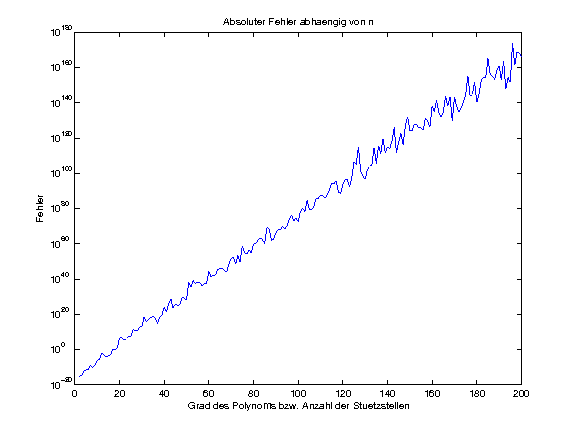
\includegraphics[width=\textwidth]{test.png}
\end{figure}

Die zugeörigen Vandermonde-Matrizen sind beliebig schlecht konditioniert, in matlab als "Infinity" berechnet.

\newpage
\item[d)] Test an $\sin$ wie auf dem Blatt. \\

\begin{lstlisting}[language=matlab]
for n = 1:200,
    f= @sin;
    % Zufaellige Stuetzstellen
    xi = pi*rand(1,n);
    p = monomialcoefficients(xi,f);
    % Fehler berechnen
    for i = 1:n,
        val(i) = abs(polyval(p,xi(i)) - f(xi(i)));
    end
    fehler(n) = max(val);
end

h = semilogy(fehler);
title('Absoluter Fehler der Interpolation in Abhaengigkeit von n');
xlabel('Grad des Polynoms n, bzw. Anzahl der Stuetzstellen');
ylabel('Maximum des Auswertungsfehlers');
saveas(h,'plotsinfehler.png');
\end{lstlisting}


\begin{figure}[h!]
\caption{Plot des Fehlers der Funktionsauswertung}
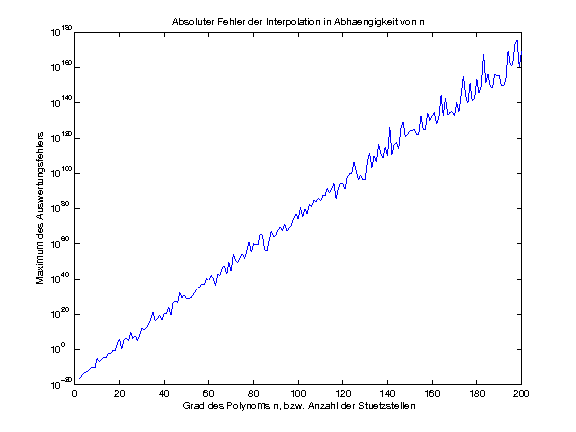
\includegraphics[width=\textwidth]{plotsinfehler.png}
\end{figure}

\pagebreak

Mit diesem Code wird Sinus und seine Interpolationen geplottet: \\

\begin{lstlisting}[language=matlab]
x = 0:0.01:2*pi;
y = sin(x);
h = plot(x,y);

title('Sinusfunktion von 0 bis 2*Pi');
saveas(h,'plotsin.png');

%%%%%%%%%%%%%%%%%%%%%%%%%%%%%%%%%%
%% Nun mit Interpolationsfunktionen:

f= @sin;

% Zufaellige Stuetzstellen
% 10 Stueck
xi10 = pi*rand(1,10);
p10 = monomialcoefficients(xi10,f);
% 20 Stueck
xi20 = pi*rand(1,20);
p20 = monomialcoefficients(xi20,f);
% 40 Stueck
xi40 = pi*rand(1,40);
p40 = monomialcoefficients(xi40,f);
% 80 Stueck
xi80 = pi*rand(1,80);
p80 = monomialcoefficients(xi80,f);

% Auswerten
x = 0:0.01:2*pi;
y10 = polyval(p10,x);
y20 = polyval(p20,x);
y40 = polyval(p40,x);
y80 = polyval(p80,x);

% Plotten
h = plot(x,y10);
title('Sinusfunktions-Interpolation von 0 bis 2*Pi mit n = 10');
saveas(h,'plotsininterpol10.png');

h = plot(x,y20,x,y40,x,y80);
title('Sinusfunktions-Interpolation von 0 bis 2*Pi mit n = 20,40,80');
saveas(h,'plotsininterpol20undmehr.png');
\end{lstlisting}

\begin{figure}[h!]
\caption{Plot der Sinusfunktion}
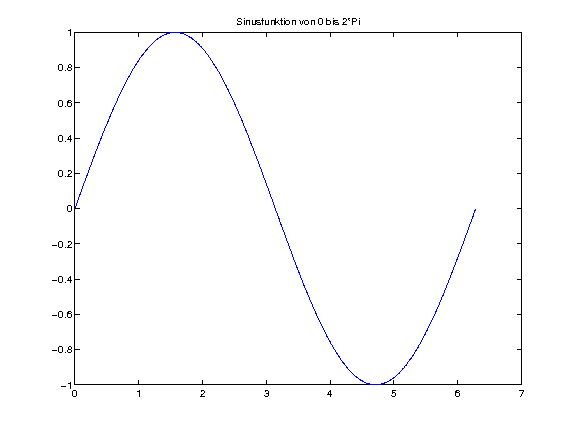
\includegraphics[width=\textwidth]{plotsin.png}
\end{figure}

\begin{figure}[h!]
\caption{Plot der Interpolation des Sinus mit 10 Stützstellen}
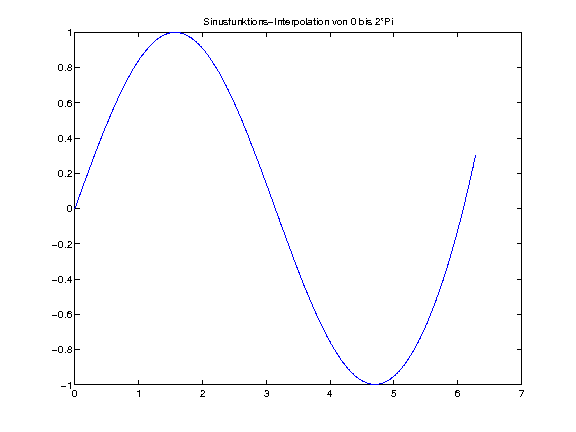
\includegraphics[width=\textwidth]{plotsininterpol.png}
\end{figure}

Die Sinus-Interpolationen mit 20, 40 und 80 Stützstellen sind sehr ungenau und wachsen extrem schnell, werden daher nicht geplottet.

\end{description}

\label{LastPage}

\end{document}
